
 \documentclass[12pt]{article}
\usepackage{graphicx}
\usepackage{booktabs}
 \usepackage{makecell}
 \usepackage{float}
 \newcommand{\diff}{\,\mathrm{d}}
\usepackage[margin=1in]{geometry}
\usepackage{fancyhdr}
\pagestyle{fancy}
\usepackage{extarrows}
\usepackage{breqn}

\newcommand{\N}{\mathbb{N}}
\newcommand{\Z}{\mathbb{Z}}
\newcommand{\trans}{^{\mathrm T}}
\usepackage{amssymb}
\usepackage[table]{xcolor}
\usepackage{bm}
\usepackage{array}
\usepackage{mathtools}
\usepackage[english]{babel}
\usepackage{natbib}
\usepackage{url}
\usepackage[utf8x]{inputenc}
\usepackage{amsmath}
\usepackage{graphicx}
\graphicspath{{images/}}
\usepackage{parskip}
\usepackage{fancyhdr}
\usepackage{vmargin}
\usepackage[font={bf, footnotesize}, textfont=md]{caption}
\usepackage{amsmath,amsthm,amssymb}


\newenvironment{theorem}[2][Theorem]{\begin{trivlist}
\item[\hskip \labelsep {\bfseries #1}\hskip \labelsep {\bfseries #2.}]}{\end{trivlist}}
\newenvironment{lemma}[2][Lemma]{\begin{trivlist}
\item[\hskip \labelsep {\bfseries #1}\hskip \labelsep {\bfseries #2.}]}{\end{trivlist}}
\newenvironment{exercise}[2][Exercise]{\begin{trivlist}
\item[\hskip \labelsep {\bfseries #1}\hskip \labelsep {\bfseries #2.}]}{\end{trivlist}}
\newenvironment{reflection}[2][Reflection]{\begin{trivlist}
\item[\hskip \labelsep {\bfseries #1}\hskip \labelsep {\bfseries #2.}]}{\end{trivlist}}
\newenvironment{proposition}[2][Proposition]{\begin{trivlist}
\item[\hskip \labelsep {\bfseries #1}\hskip \labelsep {\bfseries #2.}]}{\end{trivlist}}
\newenvironment{corollary}[2][Corollary]{\begin{trivlist}
\item[\hskip \labelsep {\bfseries #1}\hskip \labelsep {\bfseries #2.}]}{\end{trivlist}}
\DeclareMathOperator{\tr}{tr}
\DeclareMathOperator{\rank}{rank}
\DeclareMathOperator{\Span}{span}
\DeclareMathOperator{\row}{row}
\DeclareMathOperator{\col}{col}
\DeclareMathOperator{\range}{range}
\DeclarePairedDelimiterX{\inp}[2]{\langle}{\rangle}{#1, #2}
\DeclareMathOperator{\Proj}{Proj}
\DeclareMathOperator{\trace}{trace}
\newcommand{\Her}{^{\mathrm H}}
\DeclareMathOperator{\diag}{diag}
\makeatletter 
    \newcommand\fcaption{\def\@captype{table}\caption}
\makeatother
\setmarginsrb{3 cm}{2.5 cm}{3 cm}{2.5 cm}{1 cm}{1.5 cm}{1 cm}{1.5 cm}
\setlength\parindent{1em}

\title{Short Report: Large Amplitude Pendulum}                             % Title
\author{Chen Ang}                               % Author
\date{\today}                                           % Date

\makeatletter
\let\thetitle\@title
\let\theauthor\@author
\let\thedate\@date
\makeatother

\pagestyle{fancy}
\fancyhf{}
\rhead{\theauthor}
\lhead{\thetitle}
\cfoot{\thepage}

\begin{document}

%%%%%%%%%%%%%%%%%%%%%%%%%%%%%%%%%%%%%%%%%%%%%%%%%%%%%%%%%%%%%%%%%%%%%%%%%%%%%%%%%%%%%%%%%

\begin{titlepage}
    \centering
    \vspace*{0.5 cm}
    
\includegraphics[scale = 0.75,width=6cm]{CUHK}\\[1.0 cm]   % University Logo
    \textsc{\large The Chinese University of Hong Kong, Shenzhen}\\[2.0 cm]   % University Name
    \textsc{\Large PHY 1002}\\[0.5 cm]               % Course Code
    \textsc{\large Physics Laboratory}\\[0.5 cm]               % Course Name
    \rule{\linewidth}{0.2 mm} \\[0.4 cm]
    { \huge \bfseries \thetitle}\\
    \rule{\linewidth}{0.2 mm} \\[1.5 cm]
    
    \begin{minipage}{0.4\textwidth}
        \begin{flushleft} \large
            \emph{Author:}\\
            \theauthor
            \\
            \emph{Group Number:} \\
            Group 1
            \end{flushleft}
            \end{minipage}~
            \begin{minipage}{0.4\textwidth}
            \begin{flushright} \large
            \emph{Student Number:} \\
            118010009                                   % Your Student Number
            \\
            \emph{Experiment Date:}\\
            September 27, 2019
        \end{flushright}
    \end{minipage}\\[2 cm]
    
    {\large \thedate}\\[2 cm]
 
    \vfill
    
\end{titlepage}

%%%%%%%%%%%%%%%%%%%%%%%%%%%%%%%%%%%%%%%%%%%%%%%%%%%%%%%%%%%%%%%%%%%%%%%%%%%%%%%%%%%%%%%%%
%%%%%%%%%%%%%%%%%%%%%%%%%%%%%%%%%%%%%%%%%%%%%%%%%%%%%%%%%%%%%%%%%%%%%%%%%%%%%%%%%%%%%%%%%

\tableofcontents
\pagebreak


%%%%%%%%%%%%%%%%%%%%%%%%%%%%%%%%%%%%%%%%%%%%%%%%%%%%%%%%%%%%%%%%%%%%%%%%%%%%%%%%%%%%%%%%%

\rmfamily

\section{Total Momentum and Kinetic Energy in Different Collisions}
The following table records the total momentum and total kinetic energy of the system before and after four types of collisions.
\begin{table}[!htb]
	\begin{tabular}{lSSS|SSS}
		\toprule
		\multirow{2}{*}{Type} &
		\multicolumn{2}{c}{Total Momentum ($10^{-2}$ N s)} &
		\multicolumn{1}{c}{} &
		\multicolumn{2}{c}{Total Kinetic Energy (mJ)} &
		\multicolumn{1}{c}{} \\
		& {$P_0$} & {$P_f$} & {\% Diff} & {KE$_0$} & {KE$_f$} & {\% Diff} \\
		\midrule
		I.S. & 8.18 & 8.07 & -1.34 & 12.61 & 6.05 & -52.02 \\
		I.U. & 7.10& 7.32& +3.01 & 9.59& 2.56 & -73.31 \\
		E.S. & 9.75 & 9.36 & -4.00 & 17.10 & 16.80 & -1.75 \\
		E.U. & 11.60 & 10.94 & -5.69 & 25.44 & 23.03 & -9.45  \\
		\midrule
		\multicolumn{7}{c}{ I: Completely Inelastic \  E: Elastic \  S: Equal Mass \  U: Unequal Mass}\\
		\bottomrule
	\end{tabular}
\caption{Total Momentum and Kinetic Energy in Four Types of Collisions}

\end{table} 

 
\section{Plots}
This section contains graphs depicting the system in four types of collisions.



\subsection{Completely Inelastic Collision of Equal Mass}
\begin{figure}[!htb]
	\centering
	\begin{minipage}{.5\textwidth}
		\centering
		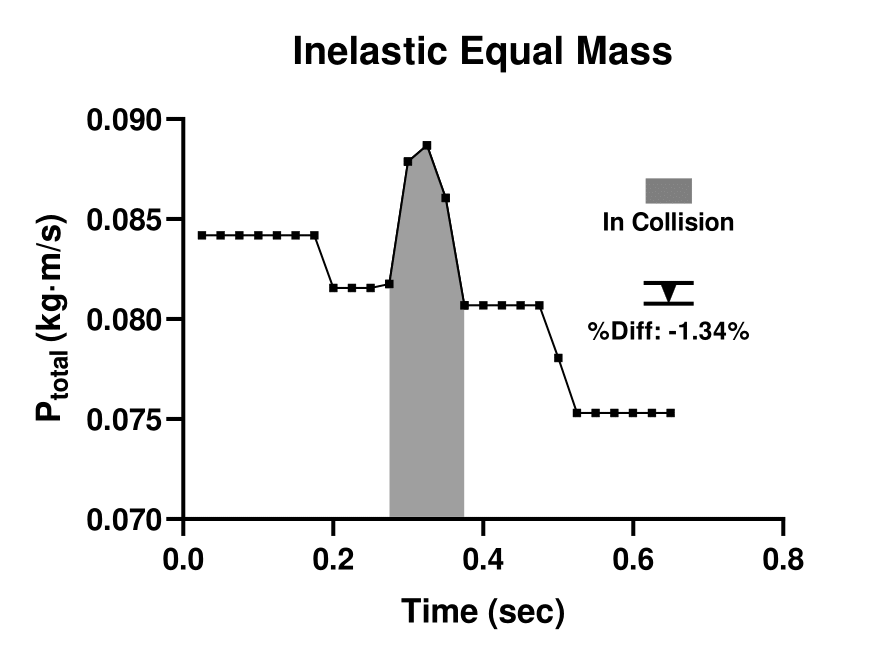
\includegraphics[width=\linewidth]{iep}
		\captionof{figure}{Total Momentum vs. Time}
		\label{fig:test1}
	\end{minipage}%
	\begin{minipage}{.5\textwidth}
		\centering
		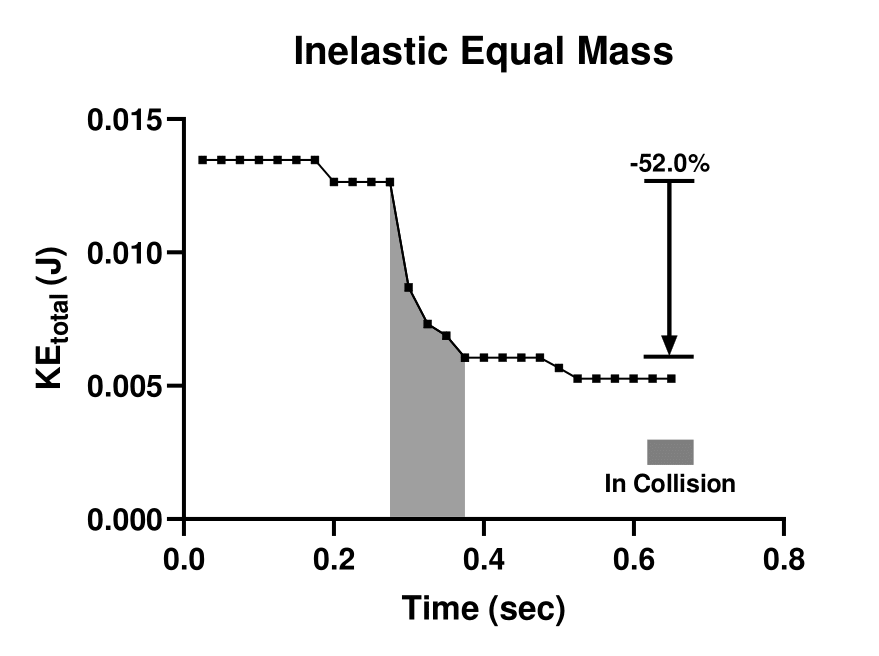
\includegraphics[width=\linewidth]{iek}
		\captionof{figure}{Total Kinetic Energy vs. Time}
		\label{fig:test2}
	\end{minipage}
\end{figure}

\subsection{Completely Inelastic Collision of Unequal Mass}
\begin{figure}[!htb]
	\centering
	\begin{minipage}{.5\textwidth}
		\centering
		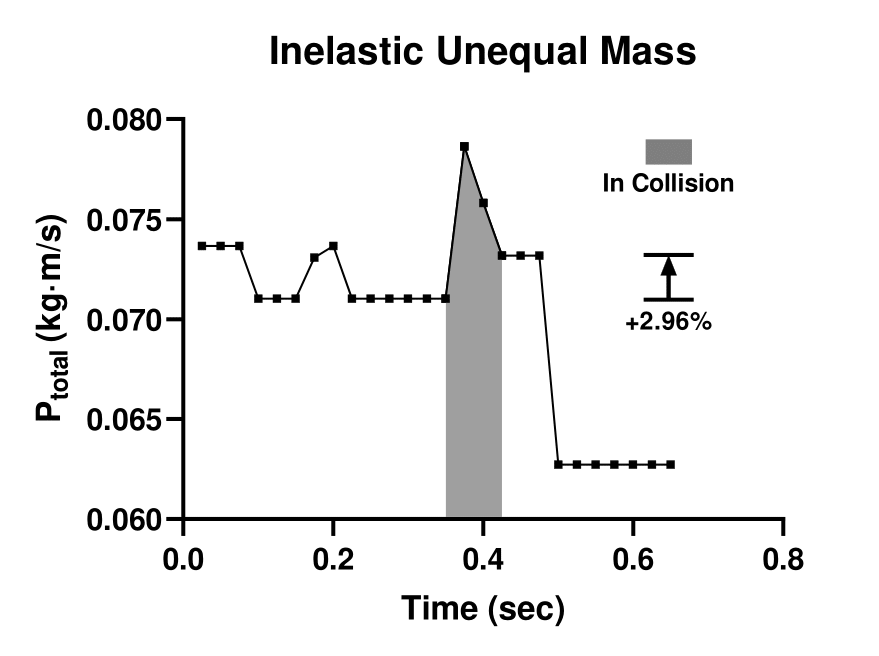
\includegraphics[width=\linewidth]{iup}
		\captionof{figure}{Total Momentum vs. Time}
		\label{fig:test1}
	\end{minipage}%
	\begin{minipage}{.5\textwidth}
		\centering
		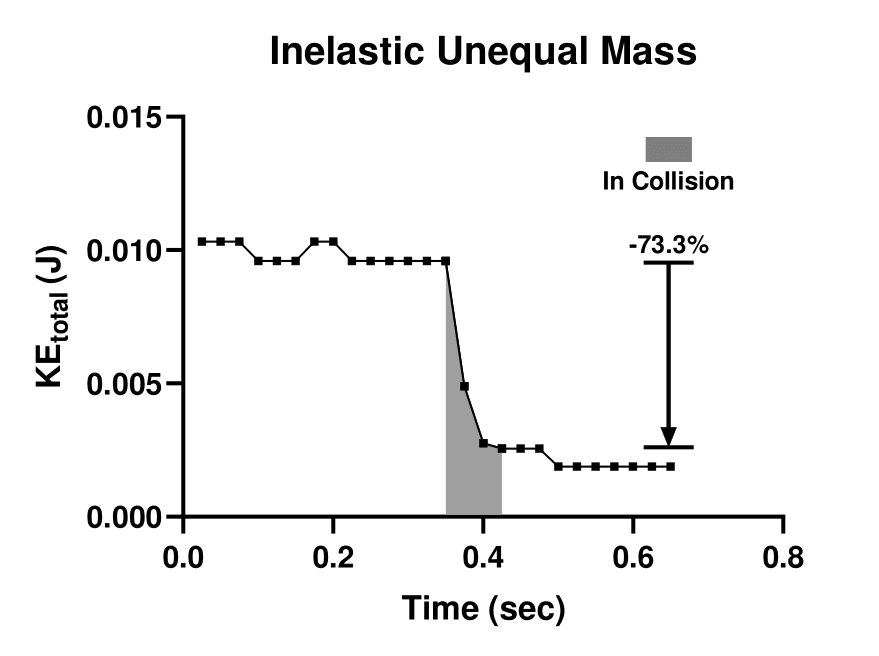
\includegraphics[width=\linewidth]{iuk}
		\captionof{figure}{Total Kinetic Energy vs. Time}
		\label{fig:test2}
	\end{minipage}
\end{figure}


\subsection{Elastic Collision of Equal Mass}
\begin{figure}[!htb]
	\centering
	\begin{minipage}{.5\textwidth}
		\centering
		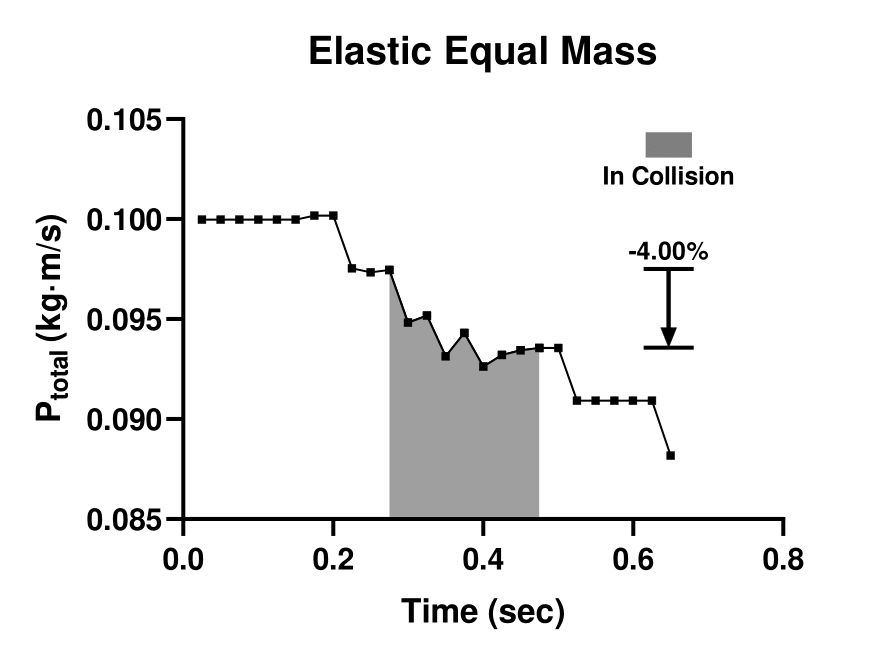
\includegraphics[width=\linewidth]{eep}
		\captionof{figure}{Total Momentum vs. Time}
		\label{fig:test1}
	\end{minipage}%
	\begin{minipage}{.5\textwidth}
		\centering
		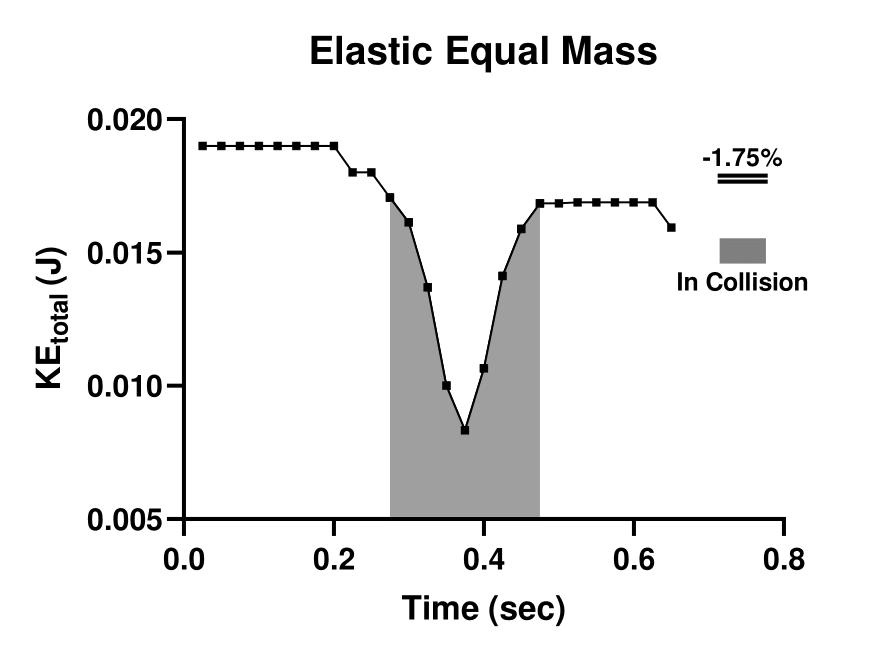
\includegraphics[width=\linewidth]{eek}
		\captionof{figure}{Total Kinetic Energy vs. Time}
		\label{fig:test2}
	\end{minipage}
\end{figure}

\newpage
\subsection{Elastic Collision of Unequal Mass}
\begin{figure}[!htb]
	\centering
	\begin{minipage}{.5\textwidth}
		\centering
		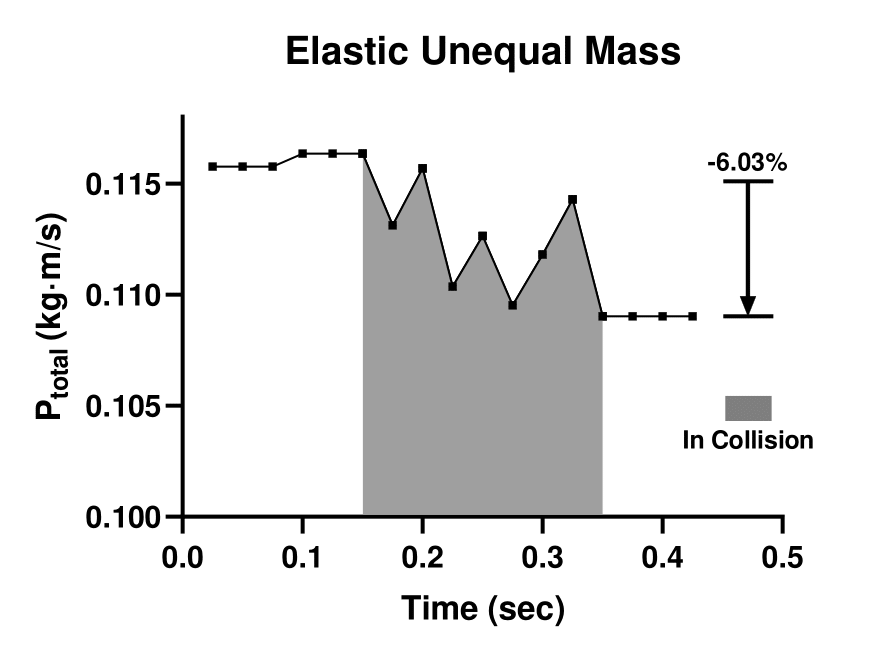
\includegraphics[width=\linewidth]{eup}
		\captionof{figure}{Total Momentum vs. Time}
		\label{fig:test1}
	\end{minipage}%
	\begin{minipage}{.5\textwidth}
		\centering
		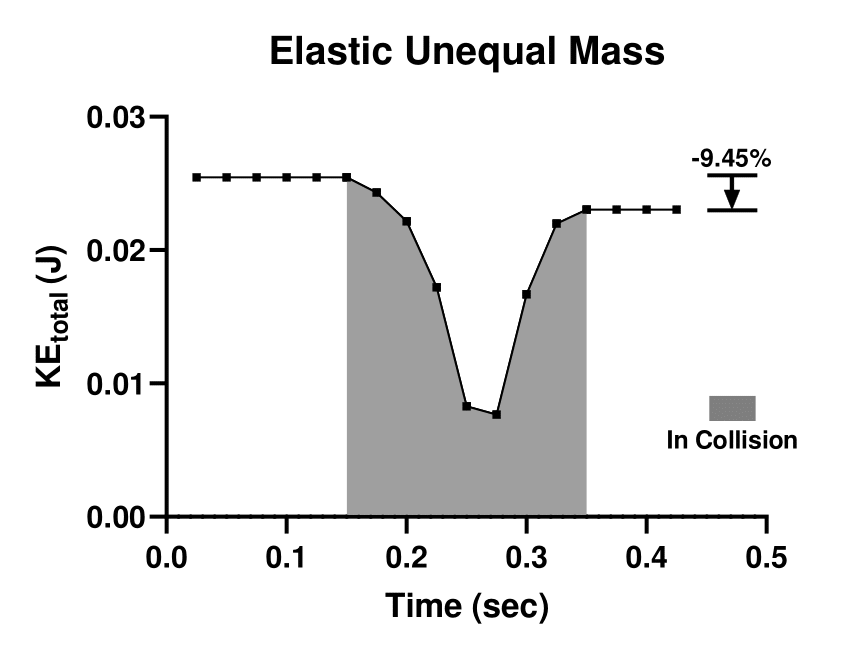
\includegraphics[width=\linewidth]{euk}
		\captionof{figure}{Total Kinetic Energy vs. Time}
		\label{fig:test2}
	\end{minipage}
\end{figure}

\section{Findings}
\subsection{Loss of Momentum and Kinetic Energy}
A loss of momentum and kinetic energy of the system outside periods of collisions is present in all cases. Since the loss of momentum appears to be linear in time, it is strongly suspected that the friction between the carts and the track, as well as the friction between the threads and the pulleys, has caused the loss of both momentum and kinetic energy.
\subsection{Momentum Conserved in All Collisions}
The percentage difference in momentum before and after the collision is small when the collision is completely inelastic (-1.34\%, +3.01\%). The difference becomes more significant in elastic collisions (-4.00\%, -5.69\%). However, it is also noticed that the period of elastic collision is about twice as long as the inelastic, which can help explain the growing difference. Since friction stays almost constant, if we double the period of collision, the negative impulse caused by friction also gets doubled. This results in a larger drop in the momentum of the system. Thus with the effect of friction filtered, momentum is likely conserved in all types of collisions.

\subsection{Kinetic Energy Conserved Only in Elastic Collisions}
The loss of kinetic energy of the system is minor in elastic collisions (-1.75\%, -9.45\%), and drastically higher in inelastic collisions (-52.02\%, -73.31\%). These results suggest that kinetic energy is conserved only in elastic collisions.
\subsection{Momentum During the Period of Collision}
The behaviors of momentum during inelastic and elastic collisions are different. During inelastic collisions, momentum first rises sharply and then falls to around the initial momentum (Figure 1, 3). This phenomenon is not yet well understood. During elastic collisions, momentum fluctuates within a short period before it reaches approximately the initial level (Figure 5, 7).
\subsection{Kinetic Energy During the Period of Collision}
The behaviors of kinetic energy during inelastic and elastic collisions are also different. During inelastic collisions, kinetic energy drops steeply without much fluctuation, as it is transformed into heat (Figure 2, 4). During elastic collisions, kinetic energy first plummets, and then goes back up to the initial level (Figure 6, 8). This behavior can be explained by the kinetic energy transforming into elastic potential energy temporarily stored in the carts, and transforming back after the collision.

\end{document}
